\subsubsection{ABN-Encoder}
\label{subsubsec:ABN-Encoder}

Der ABN-Encoder wird verwendet, um dem FOC-Regler die momentane Lage des Rotors mitzuteilen. Dazu wurde der AMT33 im Verlaufe des Projektes 5 ausgesucht und hier beschrieben. Er ist unempfindlich auf Staub, Schmutz und Öl. Die Montage und Zentrierung gestaltet sich sehr einfach. Ausserdem hat er eine einstellbar hohe Genauigkeit, auf welche beim Funktionsbeschrieb eingegangen wird. \cite[S.1]{cui_devices_cui_2019}


\paragraph{Schaltungsaufbau}\mbox{}

Nebst der 5V-Spannungsversorgung sind die Signalleitungen auf den Encoder geführt. Nämlich A, B und N. Wàhrend A und B die Codierung für die relative Wegänderung sind, gibt N an, sobald eine gesamte Umdrehung erfolgte. Auf die Schaltung innerhalb des Encoders wird nicht eingegangen.

\paragraph{Funktionsbeschrieb der Schaltung}\mbox{}

Der ABN-Encoder kann wie gesagt eine einstellbar genaue Genauigkeit ausgeben. Dies zeigt sich in einer Form der Bitanzahl pro Umdrehung. Die maximale Auflösung liegt bei 4096 Schaltvorgänge pro Umdrehung, was einer Auflösung von 12 Bit entspricht. Dies ist wichtig für die Implementierung in den FOC-Treiber. Die Ausgangspins sind normale Header-Pins. Der Spannungsausgang wurde mit einem Stützkondesator C89 versehen.

%\begin{figure}[h!]
%	\centering
%	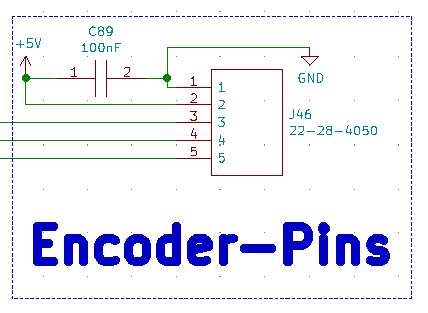
\includegraphics[width=0.5\textwidth]{graphics/Schema_ABN_Encoder}
%	\caption{Schema ABN-Encoder.}
%	\label{fig:Schema_ABN_Encoder}
%\end{figure} 